\definecolor{exxetagray}{gray}{0.75}
\definecolor{itemcolor}{RGB}{179,217,255}
\definecolor{usercolor}{RGB}{255,204,179}

\shorthandoff{"}
\chapter{Ergebnisse}
\label{ch:ergebnisse}

\section{Überblick Befragung der Mitarbeitenden}
An der Befragung der Mitarbeitenden bei EXXETA nahmen 54 Mitarbeitende aus insgesamt neun verschiedenen Teams teil.
Der Großteil der Befragten ($\approx$ 70 Prozent) stellten Mitarbeitende aus dem Team Java Enterprise Solutions dar, wobei sich die übrigen Mitarbeitenden nahezu gleichmäßg auf die anderen acht Teams (Business Application Development???) verteilt.
Die Befragung war für Mitarbeitende jedes Senioritätsniveaus und jeder Stellenbeschreibung zugängig.

% Von den 31 angefragten Fähigkeiten gaben Mitarbeitende im Mittel bei 38 Prozent der Fähigkeiten an Grundkenntnisse und bei 19 Prozent fortgeschrittene Kenntnisse zu besitzen (Werte aufgerundet auf die 2. Nachkommastelle).
% Bei knapp 43 Prozent der Fähigkeiten gaben die Befragten an, keine Kenntnisse zu besitzen.
% Von den angefragten Fähigkeiten wurden die Fähigkeiten "Backend" und "Git" von den meisten Mitarbeitenden beherrscht, während die Fähigkeit "Camunda" von den wenigsten Befragten besessen wurde.

% Von den angefragten Fähigkeiten wollten die befragten Mitarbeitenden im Durchschnitt 42 Prozent der Fähigkeiten in zukünftigen Projekten (weiter) anwenden.
% Bei 22 Prozent der Fähigkeiten gaben Mitarbeitende an, die Fähigkeit zukünftig (vorerst) nicht (weiter) anwenden zu wollen.
% Für 36 Prozent der Fähigkeiten gaben die Befragten an, der Möglichkeit, die Fähigkeit in zukünftigen Projekten anzuwenden, neutral gegenüber zu stehen.
% Übergreifend wurde die Fähigkeit "Git" von den meisten Mitarbeitenden präferiert, während die Fähigkeit "\ac{SOAP}" von den wenigsten Mitarbeitenden präferiert wurde.
% Der Fähigkeit "Helm" standen die meisten Mitarbeiter neutral gegenüber.

Abbildung \ref{fig:ergebnisse:abb1} stellt ein Tortendiagramm dar, welches die durchschnittliche Zusammensetzung der Fähigkeiten und Präferenzen eines Mitarbeitenden darstellt.
Der blau markierte Bereich stellt den Anteil der angefragten 31 Fähigkeiten dar, den ein Mitarbeitender im Mittel beherrscht (Anteile ...).
Dieser Anteil ($\approx 57$ Prozent) ergibt sich durchschnittlich aus 38 Prozent der gesamten Fähigkeiten, in denen ein Mitarbeitender Grundkenntnisse besitzt, sowie 19 Prozent der Fähigkeiten, die ein Mitarbeitender im Mittel auf dem Niveau Fortgeschritten beherrscht.
% HIER WEITERMACHEN!
Von den 31 angefragten Fähigkeiten gaben Mitarbeitende im Mittel bei mehr als der Hälfte der Fähigkeiten an diese zu beherrschen (blaue Anteile), wobei 38 Prozent der Fähigkeiten auf dem Level Grundkenntnisse und 19 Prozent auf dem Level Fortgeschritten angegeben wurden (Werte aufgerundet auf die 2. Nachkommastelle).
Dabei gaben die Befragten bei 
Bei knapp 43 Prozent der Fähigkeiten gaben die Befragten an, keine Kenntnisse zu besitzen.
\begin{figure}[H]
    \centering
	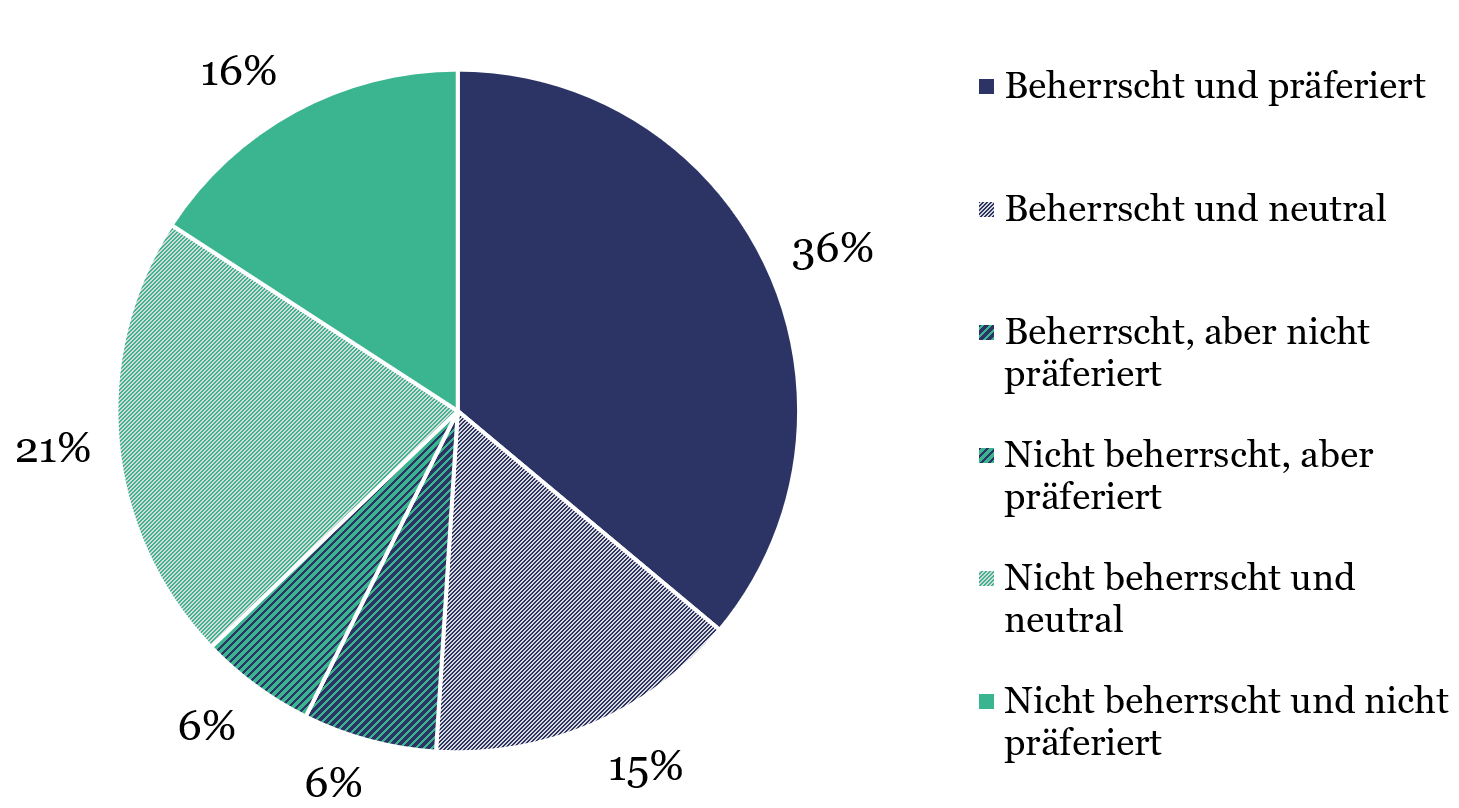
\includegraphics[width=0.9\textwidth]{gfx/verteilung-f-p.png}
	\caption[Durchschnittliche Verteilung der Fähigkeiten und Präferenzen je Mitarbeitenden]{Durchschnittliche Verteilung der Fähigkeiten und Präferenzen je Mitarbeitenden}
	\label{fig:ergebnisse:abb1}
\end{figure}

\section{Überblick Befragung der Manager}

\section{Evaluation des Algorithmus}

\shorthandon{"}